%%%%%%%%%%%%%%%%%%%%%%%%%%%%%%%%%%%%
% Slide options
%%%%%%%%%%%%%%%%%%%%%%%%%%%%%%%%%%%%

% Option 1: Slides with solutions

\documentclass[slidestop,compress,mathserif]{beamer}
\newcommand{\soln}[1]{\textit{#1}}
\newcommand{\solnGr}[1]{#1}

% Option 2: Handouts without solutions

%\documentclass[11pt,containsverbatim,handout]{beamer}
%\usepackage{pgfpages}
%\pgfpagesuselayout{4 on 1}[letterpaper,landscape,border shrink=5mm]
%\newcommand{\soln}[1]{ }
%\newcommand{\solnGr}{ }

%%%%%%%%%%%%%%%%%%%%%%%%%%%%%%%%%%%%
% Style
%%%%%%%%%%%%%%%%%%%%%%%%%%%%%%%%%%%%

\def\chp8@path{../../Chp 8}
\input{../../lec_style.tex}

%%%%%%%%%%%%%%%%%%%%%%%%%%%%%%%%%%%%
% Preamble
%%%%%%%%%%%%%%%%%%%%%%%%%%%%%%%%%%%%

\title[Lecture 33]{MA213: Lecture 33}
\subtitle{Module 5: Linear regression}
\author{OpenIntro Statistics, 4th Edition}
\institute{$\:$ \\ {\footnotesize Based on slides developed by Mine \c{C}etinkaya-Rundel of OpenIntro. \\
The slides may be copied, edited, and/or shared via the \webLink{http://creativecommons.org/licenses/by-sa/3.0/us/}{CC BY-SA license.} \\
Some images may be included under fair use guidelines (educational purposes).}}
\date{}


%%%%%%%%%%%%%%%%%%%%%%%%%%%%%%%%%%%%
% Begin document
%%%%%%%%%%%%%%%%%%%%%%%%%%%%%%%%%%%%

\begin{document}


%%%%%%%%%%%%%%%%%%%%%%%%%%%%%%%%%%%%
% Title page
%%%%%%%%%%%%%%%%%%%%%%%%%%%%%%%%%%%%

{
\addtocounter{framenumber}{-1} 
{\removepagenumbers 
\usebackgroundtemplate{\includegraphics[width=\paperwidth]{../../OpenIntro_Grid_4_3-01.jpg}}
\begin{frame}

\hfill \includegraphics[width=20mm]{../../oiLogo_highres}

\titlepage

\end{frame}
}
}


%%%%%%%%%%%%%%%%%%%%%%%%%%%%%%%%%%%%
% Recap/Agenda 
%%%%%%%%%%%%%%%%%%%%%%%%%%%%%%%%%%%%
% TODO better formatting
\begin{frame}
    \frametitle{Module 5: Linear regression}
    \begin{itemize}
        \item \hl{Previously: }Least squares regression (Chapter 8.2)
        \item \hl{This time: }Types of outliers in linear regression (Chapter 8.3)
        \item \hl{Reading: }Chapter 8.4 for next time
        \item \hl{Deadlines/Announcements: }HW 5.1 due Monday, Q4 in discussions next week
    \end{itemize}
    
\end{frame}
%%%%%%%%%%%%%%%%%%%%%%%%%%%%%%%%%%%%
% Sections
%%%%%%%%%%%%%%%%%%%%%%%%%%%%%%%%%%%%

%%%%%%%%%%%%%%%%%%%%%%%%%%%%%%%%%%%%

\section{R Demonstration: Linear regression so far}

%%%%%%%%%%%%%%%%%%%%%%%%%%%%%%%%%%%%

\section{Recap: Our tools for inference so far}

\begin{frame}
    \frametitle{Tools we already have...}
\end{frame}

%%%%%%%%%%%%%%%%%%%%%%%%%%%%%%%%%%%%

\section{Inference for linear regression}

%%%%%%%%%%%%%%%%%%%%%%%%%%%%%%%%%%%%

\subsection{Understanding regression output from software}

%%%%%%%%%%%%%%%%%%%%%%%%%%%%%%%%%%%

\begin{frame}
\frametitle{Nature or nurture?}

{\small In 1966 Cyril Burt published a paper called ``The genetic determination of differences in intelligence: A study of monozygotic twins reared together and apart". The data consist of IQ scores for [an assumed random sample of] 27 identical twins, one raised by foster parents, the other by the biological parents.}

\begin{center}
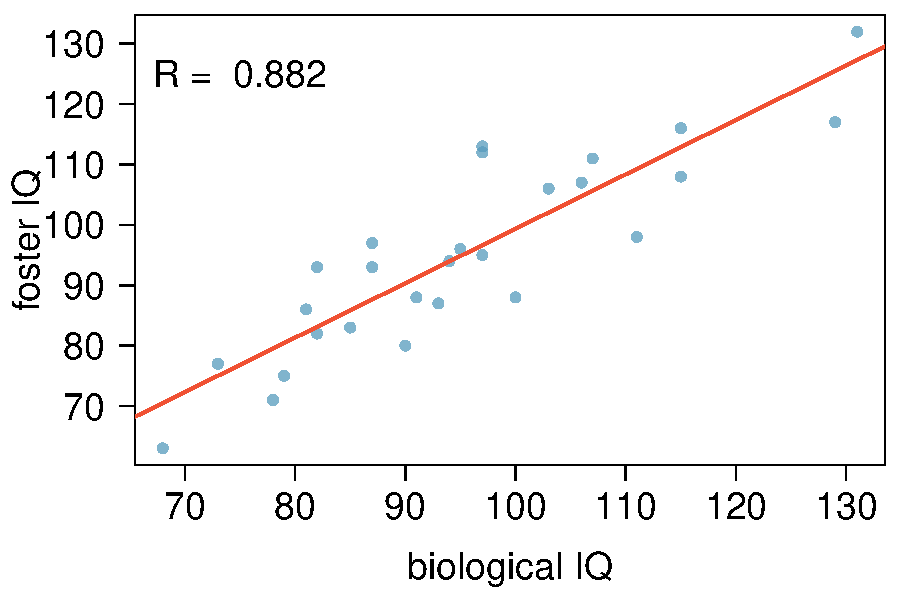
\includegraphics[width=0.7\textwidth]{\chp8@path/8-4_inf_lin_reg/figures/twins/twins_IQ}
\end{center}

\end{frame}

%%%%%%%%%%%%%%%%%%%%%%%%%%%%%%%%%%%

\begin{frame}[fragile]
\frametitle{}

\pq{Which of the following is \underline{false}?}

{\footnotesize
\begin{verbatim}
Coefficients:
                 Estimate Std. Error t value Pr(>|t|)    
(Intercept)       9.20760    9.29990   0.990    0.332    
bioIQ             0.90144    0.09633   9.358  1.2e-09

Residual standard error: 7.729 on 25 degrees of freedom
Multiple R-squared: 0.7779,	Adjusted R-squared: 0.769 
F-statistic: 87.56 on 1 and 25 DF,  p-value: 1.204e-09 
\end{verbatim}
}

\begin{enumerate}[(a)]
\item Additional 10 points in the biological twin's IQ is associated with additional 9 points in the foster twin's IQ, on average.
\solnMult{Roughly 78\% of the foster twins' IQs can be accurately predicted by the model.}
\item The linear model is $\widehat{fosterIQ} = 9.2 + 0.9 \times bioIQ$.
\item Foster twins with IQs higher than average IQs tend to have biological twins with higher than average IQs as well.
\end{enumerate}

\end{frame}

%%%%%%%%%%%%%%%%%%%%%%%%%%%%%%%%%%%

\section{Edfinity Quiz: Hypotheses for testing for the slope}  % To replace slide below, then do t-test together

%%%%%%%%%%%%%%%%%%%%%%%%%%%%%%%%%%%

\begin{frame}
\frametitle{Testing for the slope}

\pq{Assuming that these 27 twins comprise a representative sample of all twins separated at birth, we would like to test if these data provide convincing evidence that the IQ of the biological twin is a significant predictor of IQ of the foster twin. What are the appropriate hypotheses?}

\begin{enumerate}[(a)]
\item \mathhl{H_0:} $b_0 = 0$; \mathhl{H_A:} $b_0 \ne 0$ 
\item \mathhl{H_0:} $\beta_0 = 0$; \mathhl{H_A:} $\beta_0 \ne 0$ 
\item \mathhl{H_0:} $b_1 = 0$; \mathhl{H_A:} $b_1 \ne 0$ 
\solnMult{ \mathhl{H_0:} $\beta_1 = 0$; \mathhl{H_A:} $\beta_1 \ne 0$ }
\end{enumerate}

\end{frame}

%%%%%%%%%%%%%%%%%%%%%%%%%%%%%%%%%%%

\begin{frame}
\frametitle{Testing for the slope (cont.)}

{\footnotesize
\begin{center}
\begin{tabular}{rrrrr}
  \hline
 & Estimate & Std. Error & t value & Pr($>$$|$t$|$) \\ 
  \hline
(Intercept) & 9.2076 & 9.2999 & 0.99 & 0.3316 \\ 
  bioIQ & 0.9014 & 0.0963 & 9.36 & 0.0000 \\ 
   \hline
\end{tabular}
\end{center}
}

\pause

\begin{itemize}

\item We always use a $t$-test in inference for regression. $\:$ \\

\pause

\Remember{Test statistic, $T = \frac{point~estimate - null~value}{SE}$}

\pause

\item Point estimate = $b_1$ is the observed slope.

\pause

\item $SE_{b_1}$ is the standard error associated with the slope.

\pause

\item Degrees of freedom associated with the slope is $df = n - 2$, where $n$ is the sample size. $\:$ \\
\pause
\Remember{We lose 1 degree of freedom for each parameter we estimate, and in simple linear regression we estimate 2 parameters, $\beta_0$ and $\beta_1$.}

\end{itemize}

\end{frame}

%%%%%%%%%%%%%%%%%%%%%%%%%%%%%%%%%%%

\begin{frame}
\frametitle{Testing for the slope (cont.)}

{\small
\begin{center}
\begin{tabular}{rrrrr}
  \hline
 & Estimate & Std. Error & t value & Pr($>$$|$t$|$) \\ 
  \hline
(Intercept) &  9.2076 & 9.2999 & 0.99 & 0.3316 \\ 
  bioIQ & \orange{0.9014}  &   \green{0.0963} & \orange{9.36} & \textcolor{blue}{0.0000} \\ 
   \hline
\end{tabular}
\end{center}
}

\pause

\begin{eqnarray*}
T &=& \frac{\orange{0.9014} - 0}{\green{0.0963}} = \orange{9.36} \\
\pause
df &=& 27 - 2 = 25 \\
\pause
p-value &=& P(|T| > \orange{9.36}) < \textcolor{blue}{0.01}
\end{eqnarray*}

\end{frame}

%%%%%%%%%%%%%%%%%%%%%%%%%%%%%%%%%%%

\section{R Demonstration: $t$-test for the slope}

%%%%%%%%%%%%%%%%%%%%%%%%%%%%%%%%%%%


%%%%%%%%%%%%%%%%%%%%%%%%%%%%%%%%%%%%
% End document
%%%%%%%%%%%%%%%%%%%%%%%%%%%%%%%%%%%%

\end{document}